\section{BCD adder}
\FloatBarrier
\begin{enumerate}
	\item[1)]
	Vi skriver koden for to-input til to 7-segment decoders:
		\begin{lstlisting}[caption={To-input til to 7 segment decoder},label={lst:TwoBcdToTwo7SegDecoder}]
	library ieee;
	use ieee.std_logic_1164.all;
	
	entity TwoInputBCD is
	port(A, B: in std_logic_vector(3 downto 0);
	segA1, segB1: out std_logic_vector(6 downto 0));
	end TwoInputBCD;
	
	architecture selection of TwoInputBCD is
	begin
	segA1<="0000001" when (A ="0000") else
	"1001111" when (A ="0001") else
	"0010010" when (A ="0010") else
	"0000110" when (A ="0011") else
	"1001100" when (A ="0100") else
	"0100100" when (A ="0101") else
	"1100000" when (A ="0110") else
	"0001111" when (A ="0111") else
	"0000000" when (A ="1000") else
	"0001100";
	
	segB1<="0000001" when (B ="0000") else
	"1001111" when (B ="0001") else
	"0010010" when (B ="0010") else
	"0000110" when (B ="0011") else
	"1001100" when (B ="0100") else
	"0100100" when (B ="0101") else
	"1100000" when (B ="0110") else
	"0001111" when (B ="0111") else
	"0000000" when (B ="1000") else
	"0001100";
	
	end selection;
		\end{lstlisting}
	
\item[2)]
Vi overfører programmet til DE2-boardet. SW[3:0] er input A, SW[11:8] er input B, HEX4 er segA1 og HEX B er segB1. Vi sætter 0 og 0 som input som ses på figur \ref{fig:7SegDecoder00}:
	\begin{figure}[h]
		\centering
		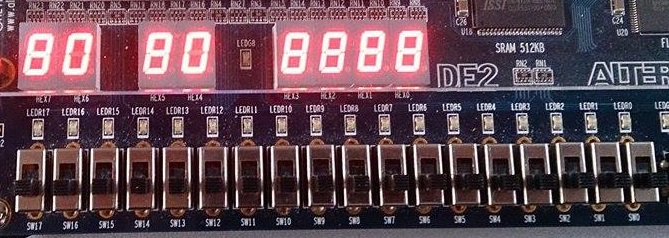
\includegraphics[scale=0.6]{pictures/Oevelse4/BCD_adder/BCD_1seg_00.jpg}
		\caption{7-segment decoder med 0 og 0 som input}
		\label{fig:7SegDecoder00}
	\end{figure}
	Vi sætter 3 og 3 som input som ses på figur \ref{fig:7SegDecoder33}:
	\begin{figure}[h]
		\centering
		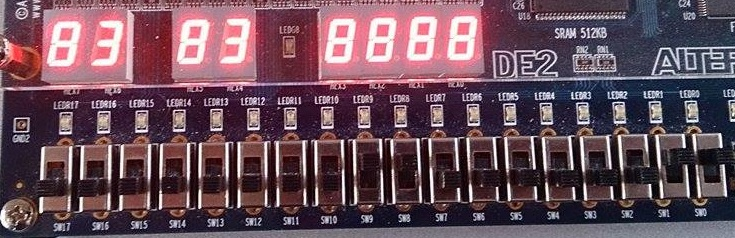
\includegraphics[scale=0.6]{pictures/Oevelse4/BCD_adder/BCD_1seg_33.jpg}
		\caption{7-segment decoder med 3 og 3 som input}
		\label{fig:7SegDecoder33}
	\end{figure}
	Vi sætter 9 og 9 som input som ses på figur \ref{fig:7SegDecoder99}:
	\begin{figure}[h]
		\centering
		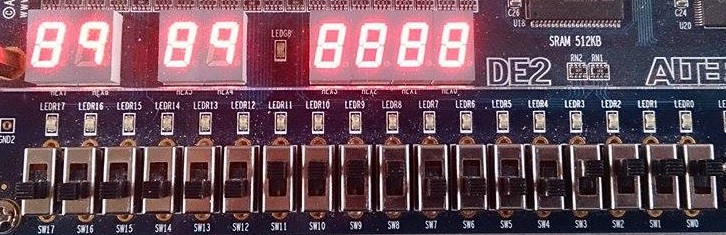
\includegraphics[scale=0.6]{pictures/Oevelse4/BCD_adder/BCD_1seg_99.jpg}
		\caption{7-segment decoder med 9 og 9 som input}
		\label{fig:7SegDecoder99}
	\end{figure}
	
\item[3)]
Vi skriver nu programmet så det udregner summen af de to inputs:
		\begin{lstlisting}[caption={To-input BCD adder},label={lst:TwoInputBCDAdder}]
library ieee;
use ieee.std_logic_1164.all;
use ieee.numeric_std.all;

entity TwoInputBCDadder is
port(A1, B1: in std_logic_vector(3 downto 0);
segA1, segB1, seg1, seg10: out std_logic_vector(6 downto 0));
end TwoInputBCDadder;

architecture selection of TwoInputBCDadder is
signal tmpsum, M : std_logic_vector(4 downto 0);
signal Asignal, Bsignal, X : std_logic_vector(3 downto 0);
signal Z : std_logic;

begin
Asignal <= "1001" when (A1 >= "1001") else A1;
Bsignal <= "1001" when (B1 >= "1001") else B1;
tmpsum <= std_logic_vector(resize(unsigned(Asignal),5) + (resize(unsigned(Bsignal),5)));
Z <= '1' when (tmpsum > "01001") else '0';
X <= "000" & Z;
M <= tmpsum when (Z = '0') else (std_logic_vector(unsigned(tmpsum) - 10));

segA1<="0000001" when (A1 ="0000") else
"1001111" when (A1 ="0001") else
"0010010" when (A1 ="0010") else
"0000110" when (A1 ="0011") else
"1001100" when (A1 ="0100") else
"0100100" when (A1 ="0101") else
"1100000" when (A1 ="0110") else
"0001111" when (A1 ="0111") else
"0000000" when (A1 ="1000") else
"0001100";

segB1<="0000001" when (B1 ="0000") else
"1001111" when (B1 ="0001") else
"0010010" when (B1 ="0010") else
"0000110" when (B1 ="0011") else
"1001100" when (B1 ="0100") else
"0100100" when (B1 ="0101") else
"1100000" when (B1 ="0110") else
"0001111" when (B1 ="0111") else
"0000000" when (B1 ="1000") else
"0001100";

seg1<="0000001" when (M = "00000") else
"1001111" when (M = "00001") else
"0010010" when (M = "00010") else
"0000110" when (M = "00011") else
"1001100" when (M = "00100") else
"0100100" when (M = "00101") else
"1100000" when (M = "00110") else
"0001111" when (M = "00111") else
"0000000" when (M = "01000") else
"0001100" when (M = "01001") else "0001100";

seg10<="0000001" when (X = "0000") else
"1001111" when (X = "0001") else "1111111";
end selection;
		\end{lstlisting}
		
\item[4)]
Vi overfører programmet til DE2-boardet. SW[3:0] er input A1, SW[11:8] er input B1, HEX4 er segA1, HEX6 er segB1, HEX0 er seg1 og HEX1 er seg10. Vi sætter 0 og 0 som input som ses på figur \ref{fig:7SegAdder0}
	\begin{figure}[h]
		\centering
		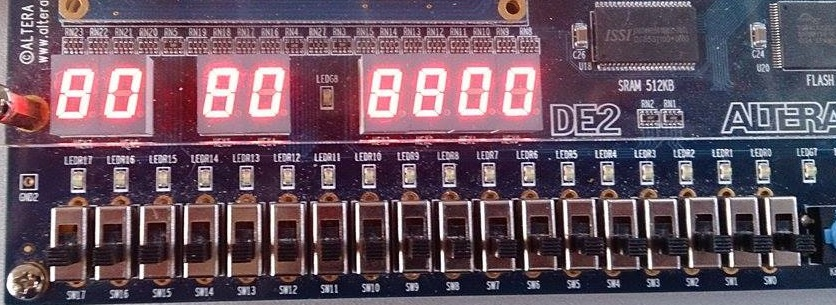
\includegraphics[scale=0.6]{pictures/Oevelse4/BCD_adder/BCD_1seg_adder_0.jpg}
		\caption{To 7-segment adder med 0 og 0 som input}
		\label{fig:7SegAdder0}
	\end{figure}
	Vi sætter 9 og 3 som input som ses på figur \ref{fig:7SegAdder12}:
	\begin{figure}[h]
		\centering
		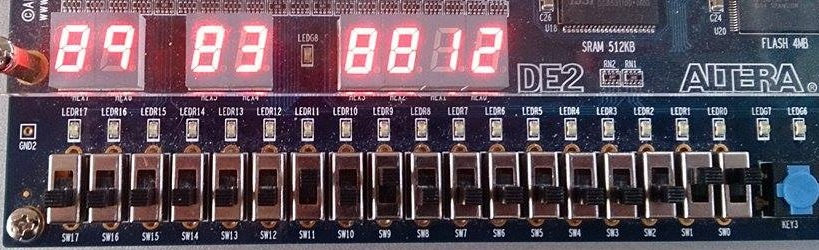
\includegraphics[scale=0.6]{pictures/Oevelse4/BCD_adder/BCD_1seg_adder_12.jpg}
		\caption{To 7-segment adder med 9 og 3 som input}
		\label{fig:7SegAdder12}
	\end{figure}
	Vi sætter ugyldige værdier som input som ses på figur \ref{fig:7SegAdderUgyldig}:
	\begin{figure}[h]
		\centering
		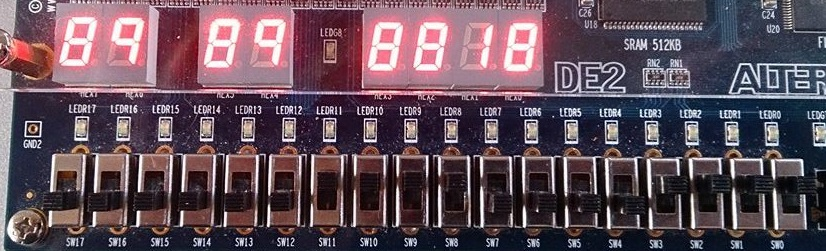
\includegraphics[scale=0.6]{pictures/Oevelse4/BCD_adder/BCD_1seg_adder_ugyldig.jpg}
		\caption{To 7-segment adder med to inputs højere end 9 (ugyldige værdier)}
		\label{fig:7SegAdderUgyldig}
	\end{figure}
\item[5)]
Vi skriver koden for en to-input BCD adder med 2-cifret input og 3-cifret output som ses i kode \ref{lst:TwoInputBCDAdder3Output}
		\begin{lstlisting}[caption={To-input BCD adder med 3-cifret output},label={lst:TwoInputBCDAdder3Output}]
library ieee;
use ieee.std_logic_1164.all;
use ieee.numeric_std.all;

entity FourInputBCDAdder is
port(A1, A10, B1, B10: in std_logic_vector(3 downto 0);
segA1, segA10, segB1, segB10, seg1, seg10, seg100: out std_logic_vector(6 downto 0));
end FourInputBCDAdder;

architecture selection of FourInputBCDAdder is
signal A1signal, A10signal, B1signal, B10signal : std_logic_vector( 3 downto 0);
signal sum1, sum10, sum100 : std_logic_vector(4 downto 0);
signal Z1, Z10 : unsigned (0 downto 0);
signal M1, M10, M100 : std_logic_vector(4 downto 0);
begin
A1signal <= "1001" when (A1 >= "1001") else A1;
A10signal <= "1001" when (A10 >= "1001") else A10;
B1signal <= "1001" when (B1 >= "1001") else B1;
B10signal <= "1001" when (B10 >= "1001") else B10;

sum1 <= (std_logic_vector(resize(unsigned(A1signal), 5) + resize(unsigned(B1signal),5)));
sum10 <= (std_logic_vector(resize(unsigned(A10signal),5)+ resize(unsigned(B10signal),5) + Z1));

Z1 <= "0" when (sum1 <= "01001" ) else "1"; 
M1 <= (std_logic_vector(unsigned(sum1) - 10)) when (Z1= "1") else sum1;

Z10 <= "0" when ( sum10 <= "01001") else "1";
M10 <= (std_logic_vector(unsigned(sum10)-10)) when (Z10= "1") else sum10;

M100 <= (std_logic_vector(("0000" & Z10)));

segA1<="0000001" when (A1signal ="0000") else
"1001111" when (A1signal ="0001") else
"0010010" when (A1signal ="0010") else
"0000110" when (A1signal ="0011") else
"1001100" when (A1signal ="0100") else
"0100100" when (A1signal ="0101") else
"1100000" when (A1signal ="0110") else
"0001111" when (A1signal ="0111") else
"0000000" when (A1signal ="1000") else
"0001100";

segA10<="0000001" when (A10signal ="0000") else
"1001111" when (A10signal ="0001") else
"0010010" when (A10signal ="0010") else
"0000110" when (A10signal ="0011") else
"1001100" when (A10signal ="0100") else
"0100100" when (A10signal ="0101") else
"1100000" when (A10signal ="0110") else
"0001111" when (A10signal ="0111") else
"0000000" when (A10signal ="1000") else
"0001100";

segB1<="0000001" when (B1signal ="0000") else
"1001111" when (B1signal ="0001") else
"0010010" when (B1signal ="0010") else
"0000110" when (B1signal ="0011") else
"1001100" when (B1signal ="0100") else
"0100100" when (B1signal ="0101") else
"1100000" when (B1signal ="0110") else
"0001111" when (B1signal ="0111") else
"0000000" when (B1signal ="1000") else
"0001100";

segB10<="0000001" when (B10signal ="0000") else
"1001111" when (B10signal ="0001") else
"0010010" when (B10signal ="0010") else
"0000110" when (B10signal ="0011") else
"1001100" when (B10signal ="0100") else
"0100100" when (B10signal ="0101") else
"1100000" when (B10signal ="0110") else
"0001111" when (B10signal ="0111") else
"0000000" when (B10signal ="1000") else
"0001100";

seg1<="0000001" when (M1 = "00000") else
"1001111" when (M1 = "00001") else
"0010010" when (M1 = "00010") else
"0000110" when (M1 = "00011") else
"1001100" when (M1 = "00100") else
"0100100" when (M1 = "00101") else
"1100000" when (M1 = "00110") else
"0001111" when (M1 = "00111") else
"0000000" when (M1 = "01000") else
"0001100" when (M1 = "01001") else "0001100";

seg10<="0000001" when (M10 = "00000") else
"1001111" when (M10 = "00001") else
"0010010" when (M10 = "00010") else
"0000110" when (M10 = "00011") else
"1001100" when (M10 = "00100") else
"0100100" when (M10 = "00101") else
"1100000" when (M10 = "00110") else
"0001111" when (M10 = "00111") else
"0000000" when (M10 = "01000") else
"0001100" when (M10 = "01001") else "0001100";

seg100<="0000001" when (M100 = "00000") else
"1001111" when (M100 = "00001") else
"0000001";
end selection;
		\end{lstlisting}

Vi overfører programmet til DE2-boardet. SW[3:0] er input A1, SW[7:4] er input A10, SW[11:8] er input B1, SW[15:12] er input B10, HEX4 er segA1, HEX6 er segB1, HEX0 er seg1, HEX1 er seg10 og HEX2 er seg100. 
\begin{figure}[h]
	Vi sætter 0 og 0 som input som ses på figur \ref{fig:BCD_2seg_adder_0}
	\centering
	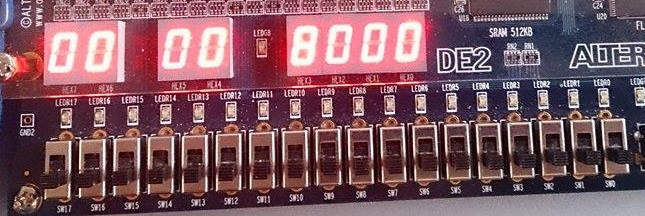
\includegraphics[scale=0.6]{pictures/Oevelse4/BCD_adder/BCD_2seg_adder_0.jpg}
	\caption{To-input BCD adder med 2-cifret input på 00 og 00 og 3-cifret output}
	\label{fig:BCD_2seg_adder_0}
\end{figure}

\begin{figure}[h]
	Vi sætter 69 og 69 som input som ses på figur \ref{fig:BCD_2seg_adder_138}:
	\centering
	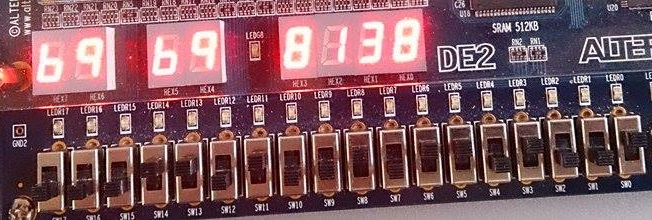
\includegraphics[scale=0.6]{pictures/Oevelse4/BCD_adder/BCD_2seg_adder_138.jpg}
	\caption{To-input BCD adder med 2-cifret input på 69 og 69 og 3-cifret output}
	\label{fig:BCD_2seg_adder_138}
\end{figure}

\begin{figure}[h]
	Vi sætter 99 og 99 som input (maksimale værdier) som ses på figur \ref{fig:BCD_2seg_adder_198}:
	\centering
	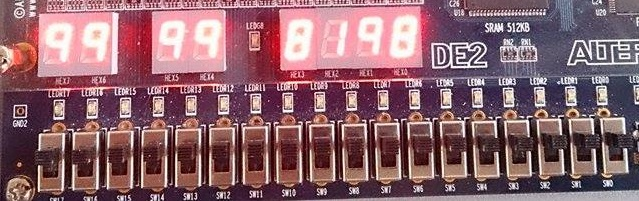
\includegraphics[scale=0.6]{pictures/Oevelse4/BCD_adder/BCD_2seg_adder_198.jpg}
	\caption{to-input BCD adder med 2-cifret input på 99 og 99 og 3-cifret output}
	\label{fig:BCD_2seg_adder_198}
\end{figure}
\end{enumerate}